%%%%%%%%%%%%%%%%%%%%%%%%%%%%%%%%%%%%%%%%%%%%%%%%%%%%%%%%%%%%%%%%%%%%%%
%     File: ExtendedAbstract_concl.tex                               %
%     Tex Master: ExtendedAbstract.tex                               %
%                                                                    %
%     Author: Andre Calado Marta                                     %
%     Last modified : 27 Dez 2011                                    %
%%%%%%%%%%%%%%%%%%%%%%%%%%%%%%%%%%%%%%%%%%%%%%%%%%%%%%%%%%%%%%%%%%%%%%
% The main conclusions of the study presented in short form.
%%%%%%%%%%%%%%%%%%%%%%%%%%%%%%%%%%%%%%%%%%%%%%%%%%%%%%%%%%%%%%%%%%%%%%

\section{Volatility}
\label{sec:vol}
Volatility is a measure of the uncertainty in future stock price movements - a higher volatility will lead to greater future fluctuations in the stock price, whereas a stock with lower volatility is more stable. This influence is represented in \autoref{fig:VarVol}.
\begin{figure}[H]
    \centering
      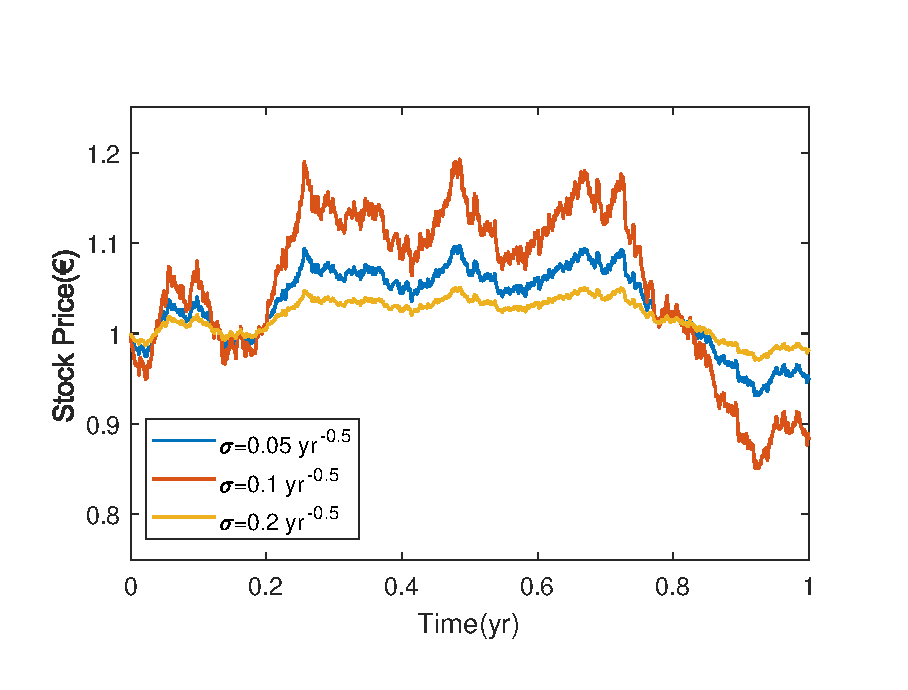
\includegraphics[width=.8\columnwidth,trim={0.6cm 0.55cm 1.35cm 1.5cm},clip]{VarVol.eps}
      \caption{Example of three identical GBM processes with different volatilities.}\label{fig:VarVol}
    \end{figure}
    
Of all the parameters in the BS model, volatility is the only one we can't easily estimate or predict, even though it has a major impact on the prices of options.

It is usually estimated empirically from the standard deviation of the historical rate of log-returns~\citep{Hull}, defined as
\begin{equation}
s=\sqrt{\frac{1}{n-1}\sum_{i=1}^n(u_i-\overline{u})^2},
\end{equation}
\noindent where the log-return rate, $u_i$, is given by
\begin{equation}
u_i=\log\left(\frac{S_i}{S_{i-1}}\right),
\end{equation}
\noindent with $\overline{u}$ defining its average and $S_i$ corresponding to the stock price at the $i$\textsuperscript{th} measurement of some given set of past observations.


Using this result, we are able to estimate the volatility of any given asset at the present moment and use it in the BS model, if we assume it remains constant in the future. The clear problem with this approach is that, when observing market data, we can see that \emph{volatilities change over time}~\citep{chourdakis}. \emph{If we try to price options assuming a constant volatility, our options will become mispriced, causing potential losses}.

Our goal is to model the instantaneous volatility (i.e. the volatility at a given point in time) and, with this model, predict its future behavior, using this knowledge to better price options.
Many models have been developed in the past, so we will only study some of the most used ones, namely Dupire's formula, where we assume that the volatility depends on the stock price and time (i.e. $\sigma=\sigma(t,S(t))$), and three other models, Heston and Static/Dynamic SABR, where the volatility itself is assumed to be a stochastic process (i.e. $\sigma=\sigma(t,S(t),W(t))$).

\subsection{Implied Volatility}
To fully understand the results shown next we need the concept of implied volatility.
\emph{Implied volatility} can be defined as the value of stock price volatility that, when input into the BS pricer in eq.\eqref{callputBS}, outputs a price equal to the market price of a given option.

Because eq.\eqref{callputBS} is not explicitly invertible w.r.t. $\sigma$, we need to use some numerical method (e.g. Newton's method) to find the value of implied volatility that matches market with model prices, i.e. we must find, numerically, the solution to the equation
\begin{equation}\label{impvolform}
C(\sigma_{imp})=C_{\mathrm{mkt}},
\end{equation}
\noindent where $C(\sigma_{imp})$ is the BS option price using $\sigma_{imp}$ as volatility and $C_{\mathrm{mkt}}$ is the price observed in the market.

It can be shown that the relation between implied volatility and option price is a monotonous increasing function, which means that we can obtain the implied volatility of an option from its price and vice versa (i.e. the relationship is bijective)~\citep{Wilmott3}. Thus, we can train our models on implied volatility data instead of using option prices, since they are equivalent.

One important property of implied volatility is that, when observing real market data, we can clearly see that it depends on the strike price, which is incompatible with the BS view (which assumes it is independent).
This phenomenon is known as the implied volatility \emph{smile} and is represented in \autoref{fig:Smile} (a \emph{skew} can also be observed for some types of underlying assets).

\begin{figure}[H]
    \centering
      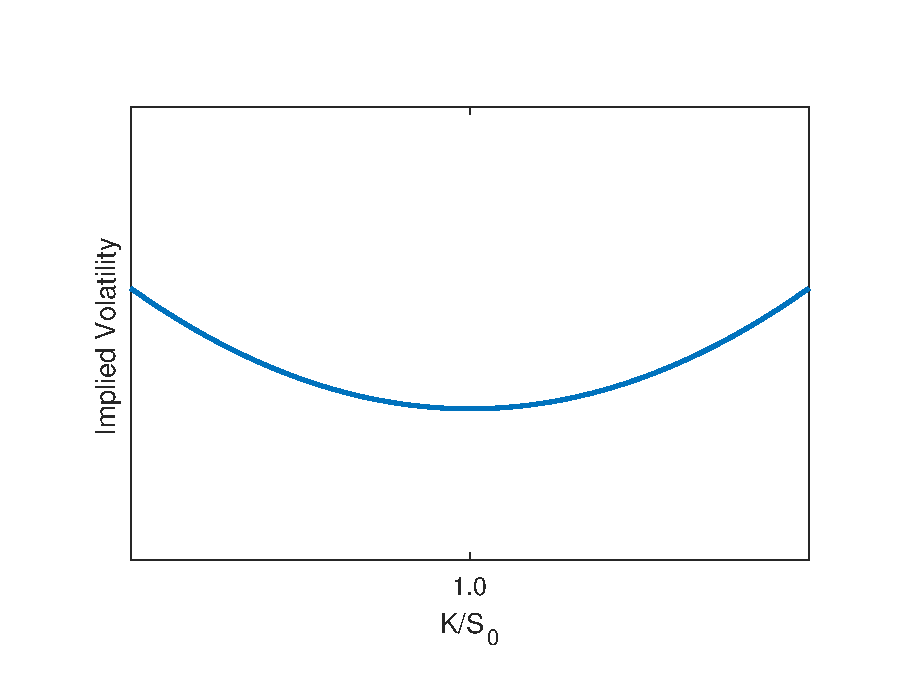
\includegraphics[width=.8\columnwidth,trim={1.35cm 0.45cm 1.4cm 1.5cm},clip]{Smile.eps}
      \caption{Implied volatility smile.}\label{fig:Smile}
    \end{figure}
    
It can also be shown that the implied volatility decreases with maturity, though this relationship is harder to define.

\subsection{Option Price Sensitivity and Vega}
When studying volatilities, it's very important to consider the sensitivity of the option price to the volatility, i.e. how a small variation in the volatility of a given option affects its price. This analysis is particularly important for volatilities because there is a high uncertainty associated with this parameter and a high sensitivity might lead to severe mispricing errors.

This sensitivity is usually called \emph{Vega}, or $\mathcal{V}$, and is defined as
\begin{equation}
\mathcal{V}=\pdv{V}{\sigma},
\end{equation}
\noindent where $V$ denotes the option price.
In particular for European calls, this value can be shown to be~\citep{Hull}
\begin{equation}
\mathcal{V}=S_0\sqrt{T}N'(d_1),
\end{equation}
\noindent where $d_1$ is given in eqs.\eqref{d1d2} and $N'(\cdot)$ is the probability density function for a standard normal distribution.

Despite its usefulness, the Vega doesn't grasp the whole picture e.g. a Vega of $4$ means that an absolute change of $2$ in the volatility produces an absolute change of $8$ in the option price - we don't have any information regarding the relative change of the price (i.e. if it changed by $1\%$ or $50\%$).
As we will see shortly, this information is indeed important. We thus define the \emph{relative change} as
\begin{equation}
\mathrm{Relative\ Change}=\pdv{V}{\sigma}\frac{\sigma}{V},
\end{equation}
\noindent where now a $\mathrm{Relative\ Change}$ of $4$ implies that a change of $2\%$ in the volatility produces a variation of $8\%$ in the option price. This relationship is plotted in \autoref{fig:Vega2}, for call options, against their strike price.
\begin{figure}[H]
    \centering
      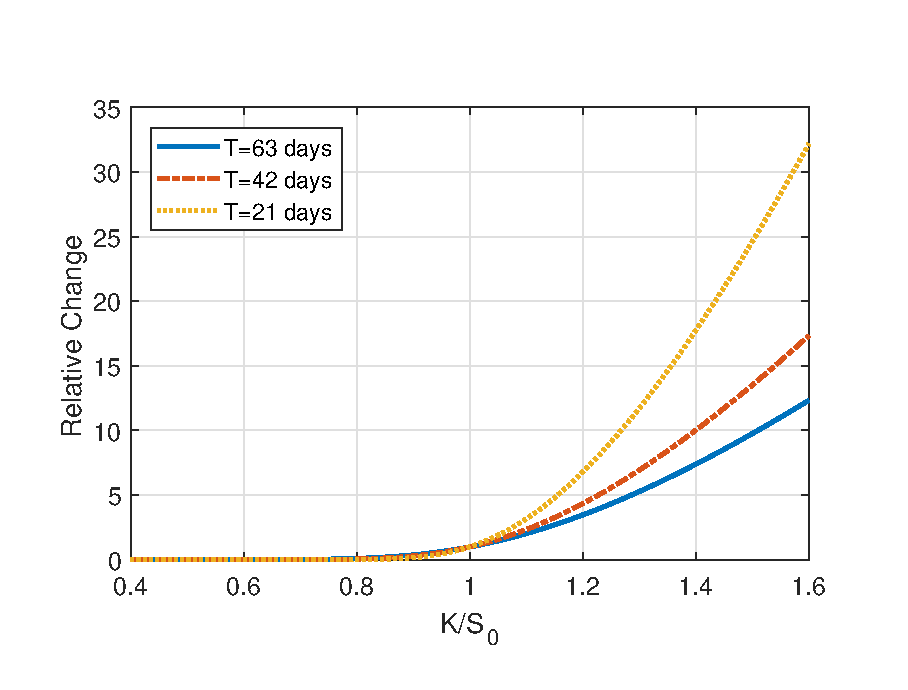
\includegraphics[width=.8\columnwidth,trim={0.7cm 0.45cm 1.1cm 1.4cm},clip]{Vega2.eps}
      \caption{Relationship between the (call) option price's relative change (w.r.t. volatility) and the respective strike prices, for different maturities.}\label{fig:Vega2}
    \end{figure}

As we can see in \autoref{fig:Vega2}, the relative change of the option price w.r.t. volatility is very large for call options with high strikes, which means that the prices of such options are very sensitive to volatility (i.e. a very slight (relative) change in the volatility will produce a very large (relative) change in the option price). It also means that the volatility is very robust w.r.t. the option price (i.e. a very large (relative) variation in the option price will barely affect the volatility).
The opposite effect is observed for call options with lower strikes, since we can see that the relative variation of the option price w.r.t. the volatility is extremely small in these cases, meaning not only that the option price is extremely robust to the volatility (i.e. a change in the volatility will barely affect the option price), but also implying that the volatility is extremely sensitive to the option price (i.e. a very slight (relative) change in the price of a call option will dramatically change its volatility).
This phenomenon will become important when we examine our results.

\subsection{Volatility Models}
As previously stated volatility is not only dynamic but also dependent on the strike price.
The (constant volatility) BS model is therefore clearly insufficient to completely grasp real-world trading and we should try to find some more appropriate volatility models.

\vspace{5pt}
\subsubsection{Dupire's Local Volatility}
One of the most used volatility models was developed by Dupire~\citep{Dupire} and uses the concept of local volatility, where we assume that volatility is a function of both time and stock price: $\sigma(S(t),t)$.
The stock price process now follows the diffusion process
\begin{equation}\label{GBM2}
dS(t)=rS(t)dt+\sigma(S(t),t)S(t)dW(t),
\end{equation}
\noindent where the local volatility, $\sigma(S(t),t)$, is a nonlinear \emph{deterministic} function of $S(t)$ and $t$.

To estimate $\sigma(S(t),t)$, we must have some implied volatility data for options with multiple strikes over multiple maturities. From this data we extract the implied volatility surface, $\sigma_{imp}(S(t),t)$, and its respective gradients w.r.t $K$ and $T$, which we can use to generate $\sigma(S(t),t)$ using

\begin{strip2}
\vspace{5pt}
\begin{equation}\label{dupire2}
\sigma(S(t),t)=\sqrt{\frac{\displaystyle\sigma_{imp}^2+2t\sigma_{imp}\pdv{\sigma_{imp}}{T}+2r(S(t))t\sigma_{imp}\pdv{\sigma_{imp}}{K}}{\displaystyle\left(1+(S(t))d_1\sqrt{t}\pdv{\sigma_{imp}}{K}\right)^2+(S(t))^2t\sigma_{imp}\left(\pdv{^2\sigma_{imp}}{K^2}-d_1\left(\pdv{\sigma_{imp}}{K}\right)^2\sqrt{t}\right)}},
\end{equation}
\end{strip2}
\noindent with $d_1$ given by
\begin{equation}
d_1=\frac{\log(S_0/S(t))+\left(r+\frac{1}{2}\sigma_{imp}^2\right)t}{\sigma_{imp}\sqrt{t}}.
\end{equation}
\noindent where we define $\sigma_{imp}=\sigma_{imp}(K,T)$ as the implied volatilities of options with maturity $T$, and strike $K$. Furthermore, $\sigma_{imp}$ and all its derivatives are evaluated at $K=S(t)$ and $T=t$.

With eq.\eqref{dupire2} we generate a local volatility surface, which we can use in eq.\eqref{GBM2} to create the respective stock price path. From this, we are able to price options, as we will see shortly.

\vspace{5pt}
\subsubsection{Heston's Stochastic Volatility}
Volatility is not constant, is not directly observable and is unpredictable. This seems to suggest that volatility is itself also a stochastic process~\citep{rebonato}.

The \emph{Heston model}, developed by Steven Heston~\citep{Heston}, is one of the most used \emph{stochastic volatility models}, and it states that stock prices satisfy the relations
\begin{equation}\label{hestons}
dS(t)=rS(t)dt+\sqrt{\nu(t)}S(t)dW_1(t),
\end{equation}
\begin{equation}\label{hestonv}
d\nu(t)=\kappa(\overline{\nu}-\nu(t))dt+\eta\sqrt{\nu(t)}dW_2(t),
\end{equation}\noindent with $\nu(t)$ corresponding to the stock price variance (i.e. the square of the volatility, $\nu(t)=(\sigma(t))^2$) and where we define $\nu_0$ as the initial variance.
Furthermore, the one-dimensional Brownian motion processes $W_1(t)$ and $W_2(t)$ have a constant correlation $\rho$, typically negative, which can be justified from market behavior~\citep{chourdakis}.

The parameters $\kappa$, $\overline{\nu}$ and $\eta$ are, respectively, the \emph{mean-reversion rate} (i.e. how fast the variance converges to its mean value), the \emph{long-term variance} (i.e. the mean value of variance) and the \emph{volatility of the variance} (i.e. how erratic is the variance process).

To appropriately use the model, we have to find the values for the parameter set $\theta=\left\{\kappa,\overline{\nu},\eta,\nu_0,\rho\right\}$ that best fit market data. For many models, this calibration process requires lengthy simulations and is impractically slow to converge. One of the reasons why the Heston model is so popular is the fact that there exists a closed-form solution that we can use to directly obtain the option prices under this model with any given parameter set $\theta$. This closed form solution (with modifications made by Schoutens~\citep{Schoutens}, Rollin \textit{et al.}~\citep{Rollin} and Cui \textit{et al.}~\citep{Cui}) is given by

\begin{strip2}
\begin{equation}\label{CH}
\begin{split}
C_{H}(K,T;\theta)&=e^{-rT}\mathbb{E}\left[\left(S(T)-K\right)\mathbbm{1}_{\left\{S(T)>K\right\}}\ \vert\ \theta\right]\\
&=e^{-rT}\left(\mathbb{E}\left[S(T)\mathbbm{1}_{\left\{S(T)>K\right\}}\ \vert\ \theta\right]-K\mathbb{E}\left[\mathbbm{1}_{\left\{S(T)>K\right\}}\ \vert\ \theta\right]\right)\\
&=S_0P_1(K,T;\theta)-e^{-rT}KP_0(K,T;\theta),
\end{split}
\end{equation}
\begin{equation}\label{P1}
P_1(K,T;\theta)=\frac{1}{2}+\frac{1}{\pi}\int_0^\infty\operatorname{Re}\left(\frac{e^{-iu\log K}}{iuS_0e^{rT}}\phi(u-i,T;\theta)\right)du,
\end{equation}
\begin{equation}\label{P2}
P_0(K,T;\theta)=\frac{1}{2}+\frac{1}{\pi}\int_0^\infty\operatorname{Re}\left(\frac{e^{-iu\log K}}{iu}\phi(u,T;\theta)\right)du,
\end{equation}
\begin{equation}
\phi(u,t;\theta)=\exp\left\{iu\left(\log S_0+rt\right)-\frac{t\kappa\overline{\nu}\rho iu}{\eta}-\nu_0A+\frac{2\kappa\overline{\nu}}{\eta^2}D\right\},
\end{equation}
\begin{equation}
D=\log \alpha+\frac{(\kappa-\alpha) t}{2}-\log\left(\frac{\alpha+\xi}{2}+\frac{\alpha-\xi}{2}e^{-\alpha t}\right),
\end{equation}
\end{strip2}
\begin{equation}
A=\frac{A_1}{A_2},
\end{equation}
\begin{equation}\label{xi}
\xi=\kappa-\eta\rho iu,
\end{equation}
\begin{equation}\label{alpha}
\alpha=\sqrt{\xi^2+\eta^2(u^2+iu)},
\end{equation}
\begin{equation}
A_1=(u^2+iu)\sinh\frac{\alpha t}{2},
\end{equation}
\begin{equation}
A_2=\alpha\cosh\frac{\alpha t}{2}+\xi\sinh\frac{\alpha t}{2}.
\end{equation}
\noindent where $C_{H}(K,T;\theta)$ corresponds to the model's European call option price, assuming a parameter set $\theta$, $i$ is the imaginary unit and where $\phi(u,t;\theta)$ is the characteristic function of the logarithm of the stock price process (the characteristic function corresponds to the Fourier transform of the probability density function of a random variable).
With this result we can easily calibrate the model by minimizing the difference between model and market prices.

\vspace{5pt}
\subsubsection{Static SABR Stochastic Volatility}
One other very commonly used stochastic volatility model was developed by Hagan \textit{et al.}~\citep{Hagan} and is known as \emph{SABR} (short for \emph{stochastic-}$\alpha\beta\rho$) (we henceforth refer to it as Static SABR to distinguish it from the Dynamic SABR model shown next). Under this model we assume that the stock price and volatility processes follow~\citep{Geeske}
\begin{equation}\label{dF}
dS(t)=rS(t)dt+e^{-r(T-t)(1-\beta)}\sigma(t)(S(t))^\beta dW_1(t),
\end{equation}
\begin{equation}\label{dsigma}
d\sigma(t)=\nu\sigma(t) dW_2(t),
\end{equation}
\noindent where $\alpha=\sigma(0)$ and, as before, the two Brownian motion processes $W_1(t)$ and $W_2(t)$ have a \emph{constant} correlation of $\rho$.

The parameters $\beta$ and $\nu$ correspond, respectively to the \emph{skewness} (i.e. how the volatility smile moves when the stock price changes) and the \emph{volatility of volatility} (i.e. how erratic is the volatility process).

As for the Heston model, in Static SABR we also have a (quasi-)closed form solution from which we can extract the option's implied volatility for any given parameter set (the respective price can be obtained with eq.\eqref{impvolform}). This formula is given by (with modifications made by Oblój~\citep{Obloj})

\newpage

\begin{strip2}
\begin{equation}\label{sabr}
\begin{split}
\sigma_{StatSABR}(K,f,T)\approx&\frac{1}{\displaystyle\left[1+\frac{(1-\beta)^2}{24}\log^2\left(\frac{f}{K}\right)+\frac{(1-\beta)^4}{1920}\log^4\left(\frac{f}{K}\right)\right]}.\left(\frac{\nu\log\left(f/K\right)}{x(z)}\right)\\
&.\left\{1+T\left[\frac{(1-\beta)^2}{24}\frac{\alpha^2}{(Kf)^{1-\beta}}+\frac{1}{4}\frac{\rho\beta\nu\alpha}{(Kf)^{(1-\beta)/2}}+\frac{2-3\rho^2}{24}\nu^2\right]\right\},
\end{split}
\end{equation}
\end{strip2}
\noindent with $z$ and $x(z)$ defined as
\begin{equation}
z=\frac{\nu\left(f^{1-\beta}-K^{1-\beta}\right)}{\alpha(1-\beta)},
\end{equation}
\begin{equation}
x(z)=\log\left\{\frac{\sqrt{1-2\rho z+z^2}+z-\rho}{1-\rho}\right\},
\end{equation}
\noindent using $f=S_0e^{rT}$.

We again need to find the optimal values for the parameters that best fit the market data.

\vspace{5pt}
\subsubsection{Dynamic SABR Stochastic Volatility}
One of the main setbacks of the Static SABR model is the fact that it behaves badly when we try to fit options with different maturities~\citep{Hagan}. To solve this, the authors developed an alternative model, known as \emph{Dynamic SABR}, similar to the Static SABR model but where we replace the parameters $\nu$ and $\rho$ with some functions of time, $\nu(t)$ and $\rho(t)$, chosen empirically.

Fernandez \textit{et al.}~\citep{Fernandez} claimed that $\nu(t)$ and $\rho(t)$ should tend to zero with time. In this work, we will use the functions suggested by those authors
\begin{equation}\label{rhot}
\rho(t)=\rho_0e^{-at},
\end{equation}
\begin{equation}\label{nut}
\nu(t)=\nu_0e^{-bt},
\end{equation}
\noindent with $\rho_0\in[-1,1]$, $\nu_0>0$, $a>0$ and $b>0$.

For this particular choice of $\nu(t)$ and $\rho(t)$, the Dynamic SABR model also has a (quasi-)closed form solution, which we can use to directly obtain the option's implied volatility with any given parameter set. This formula (with some modifications made by Osajima~\citep{Osajima}) is given by 

\begin{strip2}
\vspace{5pt}
\begin{equation}\label{dynsabr}
\sigma_{DynSABR}(K,f,T)=\frac{1}{\omega}\left(1+A_1(T)\log\left(\frac{K}{f}\right)+A_2(T)\log^2\left(\frac{K}{f}\right)+B(T)T\right),
\end{equation}
\begin{equation}
A_1(T)=\frac{\beta-1}{2}+\frac{\eta_1(T)\omega}{2},
\end{equation}
\begin{equation}
A_2(T)=\frac{(1-\beta)^2}{12}+\frac{1-\beta-\eta_1(T)\omega}{4}+\frac{4\nu_1^2(T)+3(\eta_2^2(T)-3\eta_1^2(T))}{24}\omega^2,
\end{equation}
\begin{equation}
B(T)=\frac{1}{\omega^2}\left(\frac{(1-\beta)^2}{24}+\frac{\omega\beta\eta_1(T)}{4}+\frac{2\nu_2^2(T)-3\eta_2^2(T)}{24}\omega^2\right),
\end{equation}
\begin{equation}
\nu_1^2(T)=\frac{6\nu_0^2}{(2bT)^3}\left[\left(\frac{(2bT)^2}{2}-2bT+1\right)-e^{-2bT}\right],
\end{equation}
\begin{equation}
\nu_2^2(T)=\frac{12\nu_0^2}{(2bT)^3}\left[e^{-2bT}(1+bT)+bT-1\right],
\end{equation}
\begin{equation}
\eta_1(T)=\frac{2\nu_0\rho_0}{T^2(a+b)^2}\left[(a+b)T+e^{-(a+b)T}-1\right],
\end{equation}
\begin{equation}
\eta_2^2(T)=\frac{3\nu_0^2\rho_0^2}{T^4(a+b)^4}\left[e^{-2(a+b)T}-8e^{-(a+b)T}+(7+2T(a+b)(-3+(a+b)T))\right].
\end{equation}
\end{strip2}
\noindent where $f=S_0e^{rT}$ and $\omega=f^{1-\beta}/\alpha$.